\documentclass{article}

%used package
\usepackage[]{graphicx}
\usepackage[utf8]{inputenc}
%package for code
\usepackage{listings}
\usepackage{wrapfig}

% Adds hyperlinks to references
\usepackage{hyperref}

\usepackage[italian]{babel}

% If multiple images are to be added, a folder (path) with all the images can be added here 
\graphicspath{{images/}}

\usepackage[left=80pt,right=80pt]{geometry}

\begin{document}

%Adds the title page
\begin{titlepage}
	\centering
	{\large Laboratorio di Reti - Corso A \par}
	\vspace{1.5cm}
	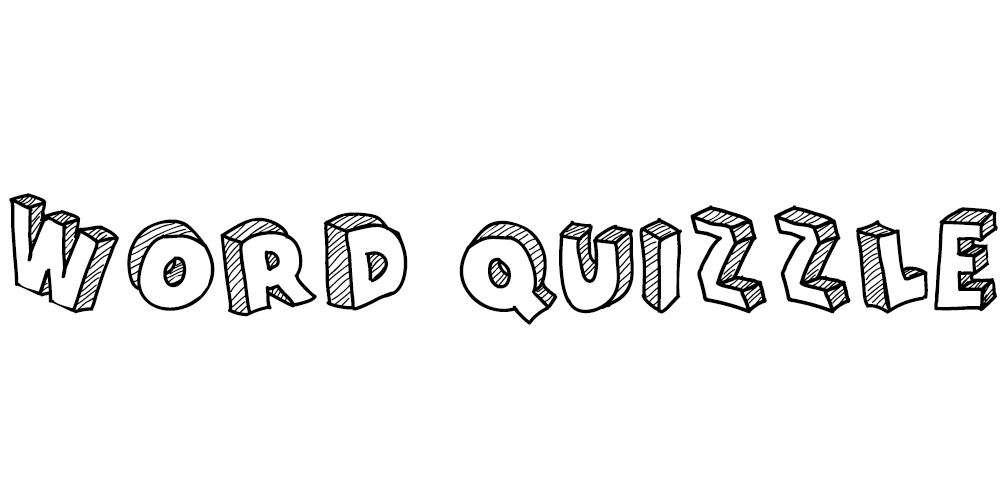
\includegraphics[scale=0.3]{quizzlelogolong.png} \\
	{\large \textbf{documentazione riguardante scelte implementative e protocollo messaggi} \par}
	\vspace{4cm}
	{\large Docente: Laura Ricci \\
	        Studente: Raffaele Apetino, Matricola 549220 \par}
	\vspace{1.3cm}

    
\includegraphics[scale=1]{universitapisa.png}
    
    \vspace{1.3cm}
    
	% Information about the University
	{\normalsize Dipartimento di Informatica \par}
		
	% Set the date
	{\normalsize 30-01-2020 \par}
	
	\pagebreak

\end{titlepage}

% Adds a table of contents
\tableofcontents{}
\clearpage

\section{Introduzione}
Il progetto riguarda la creazione di un sistema di sfide di traduzione (italiano-inglese) basato sulla struttura Client-Server utilizzando il linguaggio Java. E' richiesto anche di gestire una rete sociale in cui gli utenti possono registrarsi, aggiungere amicizie, confrontarsi attraverso classifiche di punteggio e altro. Tutto comincia con la registrazione degli utenti tramite Remote Method Invocation, segue il dialogo tra client e server secondo connessione TCP (che chiameremo TCP standard). La sfida sfrutta anch'essa TCP (la chiameremo invece TCP sfida). Mentre per le notifiche di sfida tra due utenti è stato richiesto di usare UDP. Le traduzioni si basano sulla API offerta dal servizio gratuito \href{https://mymemory.translated.net/doc/spec.php}{MyMemory}. \\
L'interfaccia grafica è stata creata sfruttando il framework \href{https://docs.oracle.com/javase/8/javafx/get-started-tutorial/jfx-overview.htm}{JavaFX} e \href{https://gluonhq.com/products/scene-builder/}{SceneBuilder}, quest'ultimo è un applicativo che permette la creazione dei file FXML (an XML-based user interface markup language created by Oracle for defining the user interface of a JavaFX application)\cite{FXMLwiki} attraverso semplici drag and drop, crop e resize dei vari elementi che compongono l'interfaccia. I file FXML in output sono poi caricabili tramite classi apposite di JavaFX come la classe FXMLLoader. Per la gestione dei file di persistenza, contenti le informazioni delle strutture dati del server, ho utilizzato il formato JSON con l'aiuto della libreria di Google \href{https://github.com/google/gson/blob/master/UserGuide.md}{Gson} e \href{https://code.google.com/archive/p/json-simple/}{JSON.simple}.

\section{Istruzioni per Compilazione e Avvio}
Il progetto è stato testato su ambienti MacOS e Linux (distr. Ubuntu). Di fondamentale importanza usare per la compilazione un JDK 8 o maggiore, poichè esso contiene nativamente JavaFX. (nel mio caso ho utilizzato Java 9.0.1).\\
Comandi per compilazione:
\begin{lstlisting}[language=bash]
javac -cp ".:~/jars/json-simple-1.1.jar:~/jars/gson-2.8.6.jar:" WQServer.java
javac -cp ".:~/jars/json-simple-1.1.jar:~/jars/gson-2.8.6.jar:" WQClient.java
\end{lstlisting}

Comandi per esecuzione:
\begin{lstlisting}[language=bash]
java -cp ".:~/jars/json-simple-1.1.jar:~/jars/gson-2.8.6.jar:" WQServer
java -cp ".:~/jars/json-simple-1.1.jar:~/jars/gson-2.8.6.jar:" WQClient
\end{lstlisting}
\clearpage

\section{WQServer}
Il server appena partito si occupa di creare l'istanza del WQDatabase (o ricreare partendo dai file di persistenza), in seguito dopo aver creato ed esportato il registry per la registrazione tramite RMI si mette in ascolto sulla socket in un ciclo dove accetta i vari client che vogliono connettersi ad esso. Per limitare il numero di client collegati il server sfrutta un Thread Pool Executor con LinkedBlockingQueue. Questo permette di porre un limite al numero massimo di thread che una singola macchina può gestire (se è l'unica istanza dell'applicativo che gira sull'host) evitando così la creazione di infiniti thread ed il collasso della macchina. Dopo l'accettazione del client sulla socket viene eseguito un WQTask che si occuperà di quel singolo client fino al momento di logout dell'utente. Nel caso in cui la pool sia al completo il client aspetta nella coda (la quale è possibile condividere attraverso framework come terracotta e quindi facilemente scalabile).

% A  after the section/chapter command indicates an unnumbered header which will not be added to the table of contents
\subsection{Protocollo di comunicazione standard}
Come detto precedentemente la registrazione dell'utente avviene tramite RMI, invece la sintassi dei messaggi inviati dal client al server della comunicazione TCP standard è così definito: (differisce dal protocollo TCP sfida)

\begin{table}[h]
\centering
\begin{tabular}{l|l|l|l|l}
LOGIN  & USERNAME   & PASSWORD   & HOSTADDRESS & UDPPORT  \\
ADD    & USERNAME   & NICKFRIEND &             &          \\
REMOVE & USERNAME   & NICKFRIEND &             &          \\
POINTS & USERNAME   &            &             &          \\
LIST   & USERNAME   &            &             &          \\
RANK   & USERNAME   &            &             &          \\
CHALL  & CHALLENGER & CHALLENGED &             &          \\
LOGOUT & USERNAME   &            &             &         
\end{tabular}
\end{table}

\subsubsection{Codici di Errore}
Codici inviati dal Server al Client sotto connessione TCP standard.
\begin{table}[h]
\centering
\begin{tabular}{l|l}
9  & Operazione non valida                 \\
10 & Registrazione OK                      \\
11 & Username già presente                 \\
12 & Login OK                              \\
13 & Password Errata                       \\
14 & Utente Inesistente                    \\
15 & Utente già online                     \\
16 & Logout OK                             \\
17 & Già presente nella lista di amicizie  \\
18 & Aggiunto amico                        \\
19 & Non presente nella lista amicizie                     \\
20 & Rimozione amicizia OK                 \\
21 & Invio richiesta sfida                 \\
22 & Utente non online                    
\end{tabular}
\end{table}

\subsection{WQTask}
Ad ogni client è associato un thread apposito che gestirà tutte le sue richieste, la struttura è un ciclo che legge sequenzialmente le richieste del client arrivate secondo protocollo e le tokenizza. Ad ogni richiesta il thread chiama i rispettivi metodi di WQDatabase, classe definita per gestire tutti i dati. 

\subsection{WQDatabase}
E' la classe fulcro del server, in essa sono contenute le strutture dati che contengono tutte le informazioni dei giocatori, è la classe che si occupa di aggiornare i file JSON di persistenza associati alle strutture e contiene i metodi per aggiornare e controllare i dati. Le due strutture principali sono:
\begin{lstlisting}[language=Java]
private HashMap<String, String> passwords;
private HashMap<String, WQUser> users;
\end{lstlisting}
La prima è una HashMap che ha come chiave il nome utente e come valore la password salvata come hashing one-way SHA-256 concatenando username e password. Questo permette sicurezza nel caso in cui il file di persistenza passwords.json venga raggiunto da chi non è di competenza. Il concatenamento dell'username e della password permette di avere due immagini hash diverse nell'eventualità che due utenti scelgano la stessa password. \\
La seconda struttura invece si occupa di tenere in memoria tutti gli utenti del gioco, ha come chiave il nome utente e come valore una istanza di WQUser (definito nella prossima sottosezione). 
Il metodo costruttore di WQDatabase si occupa, nel caso in cui i file di persistenza siano presenti, di ricreare tutte le istanze delle due strutture sfruttando la libreria Gson. I file di persistenza vengono aggiornati nel caso in cui un utente si registri, aggiunga o rimuova un amico o quando i punti dell'utente cambino (avviene al termine della sfida). Questa scelta può risultare computazionalemte costosa ma sicura nel caso di crash da parte del server, poichè i dati rimangono consistenti. Una soluzione alternativa potrebbe essere la creazione di un thread apposito che ogni tot tempo si occupi di aggiornare i file JSON.

\subsection{WQUser}
Classe che si occupa di rappresentare gli utenti/giocatori di WordQuizzle. In essa sono contenute le variabili per salvare l'indirizzo IP del client, la porta UDP per le notifiche, punteggio , lo stato (online/offline) e la lista delle amicizie. Quest'ultima è definita come un ArrayList di stringhe (username), per ottenere quindi le informazioni degli amici è necessario eseguire una ricerca nella HashTable con chiave username (costo 0(1) * O(dimLista)). La classe implementa Comparable, poichè gli utenti dovranno essere comparati secondo la variabile contentente i punti, per poter creare la classifica.

\section{WQClient}
Il client è composto principalmente da due thread. Il thread principale si occupa di gestire l'interfaccia grafica, dopo aver ottenuto il registry del server fa partire la User Interface chiamando il metodo launch() definito da JavaFX (notare come WQClient estenda Application, classe definita dal framework). Il metodo launch() chiamerà a sua volta il metodo start() che si occuperà di creare lo "stage". Viene poi caricato il file FXML della scena di login (creato con SceneBuilder) usando FXMLLoader, infine viene associato il Controller della scena (RegisterLoginController). L'interfaccia grafica da questo momento in poi ciclerà attraverso le varie "scene" per la schemata principale (con controller MainViewController) e il gioco (GameViewController). "A controller is a compiled class that implements the "code behind" the object hierarchy defined by the document." \cite{javafxDocumentation} Il compito del Controller è quindi quello di associare ogni ID (associazione tra elemento e ID avviene in SceneBuilder) e il codice che deve essere eseguito quando l'evento occorre (ad esempio click su un tasto). Tutti i Controller hanno un riferimento alla classe WQClient, in essa sono definiti tutti i metodi "handler" che si occupano di comunicare con il server tramite socket TCP standard.

\subsection{RegisterLoginController}
\begin{center}
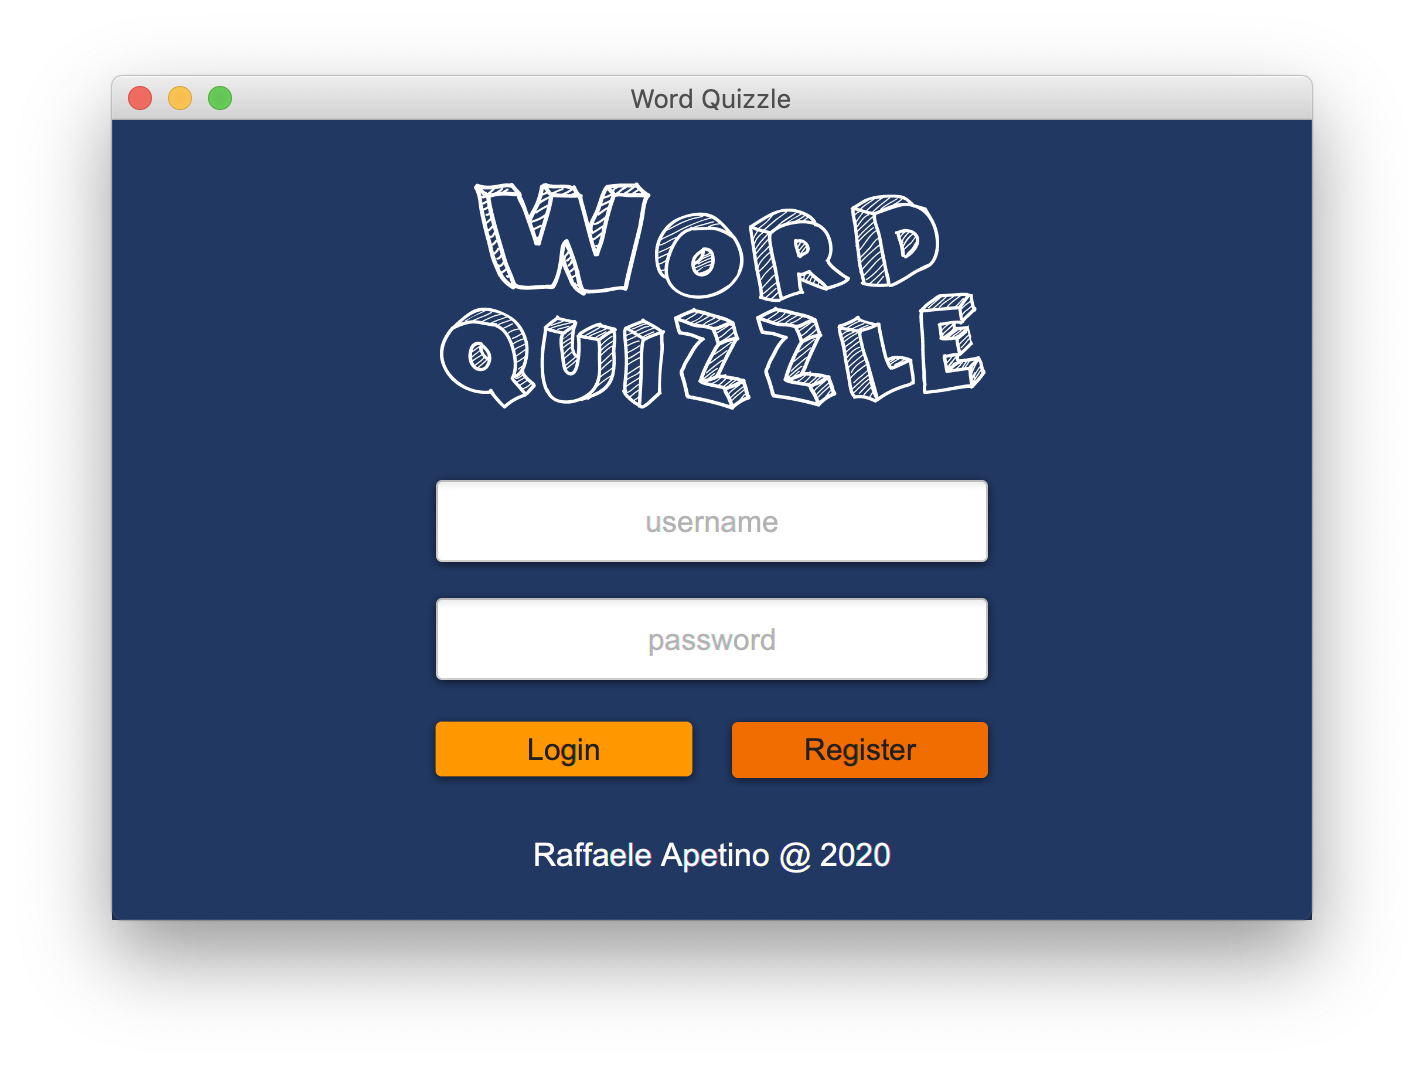
\includegraphics[scale=0.5]{quizzleloginregister.png}
\end{center}
Il controller per la registrazione e il login contiene due TextField, una Label e due Button. Le TextField sono passive, cioè non fanno parte di quegli elementi che aggiungono eventi alla Event Queue. Per gestire l'evento di click dei due bottoni ho definito due metodi:
\begin{itemize}
    \item registerbtnAction: gestisce il tasto di registrazione, chiama il metodo RMI della registry passando come parametro i due campi delle TextField.
    \item loginbtnAction: gestisce il tasto di login, chiama il metodo login handler di WQClient passando come parametro i due campi delle TextField. Il metodo login\textunderscore handler si occupa di creare un collegamento TCP con il server, invia la stringa di login secondo protocollo di comunicazione standard. In caso di login corretto crea la socket UDP e manda in esecuzione un thread che si occuperà di ricevere le notifiche di sfida. (Tutto ciò che riguarda la sfida e notifiche è descritta nel capitolo Sfida). 
\end{itemize}
Entrambi, in caso di errore, settano la label (posizionata sotto i due tasti) con la stringa associata al codice di errore.

\subsection{MainViewController}
\begin{center}
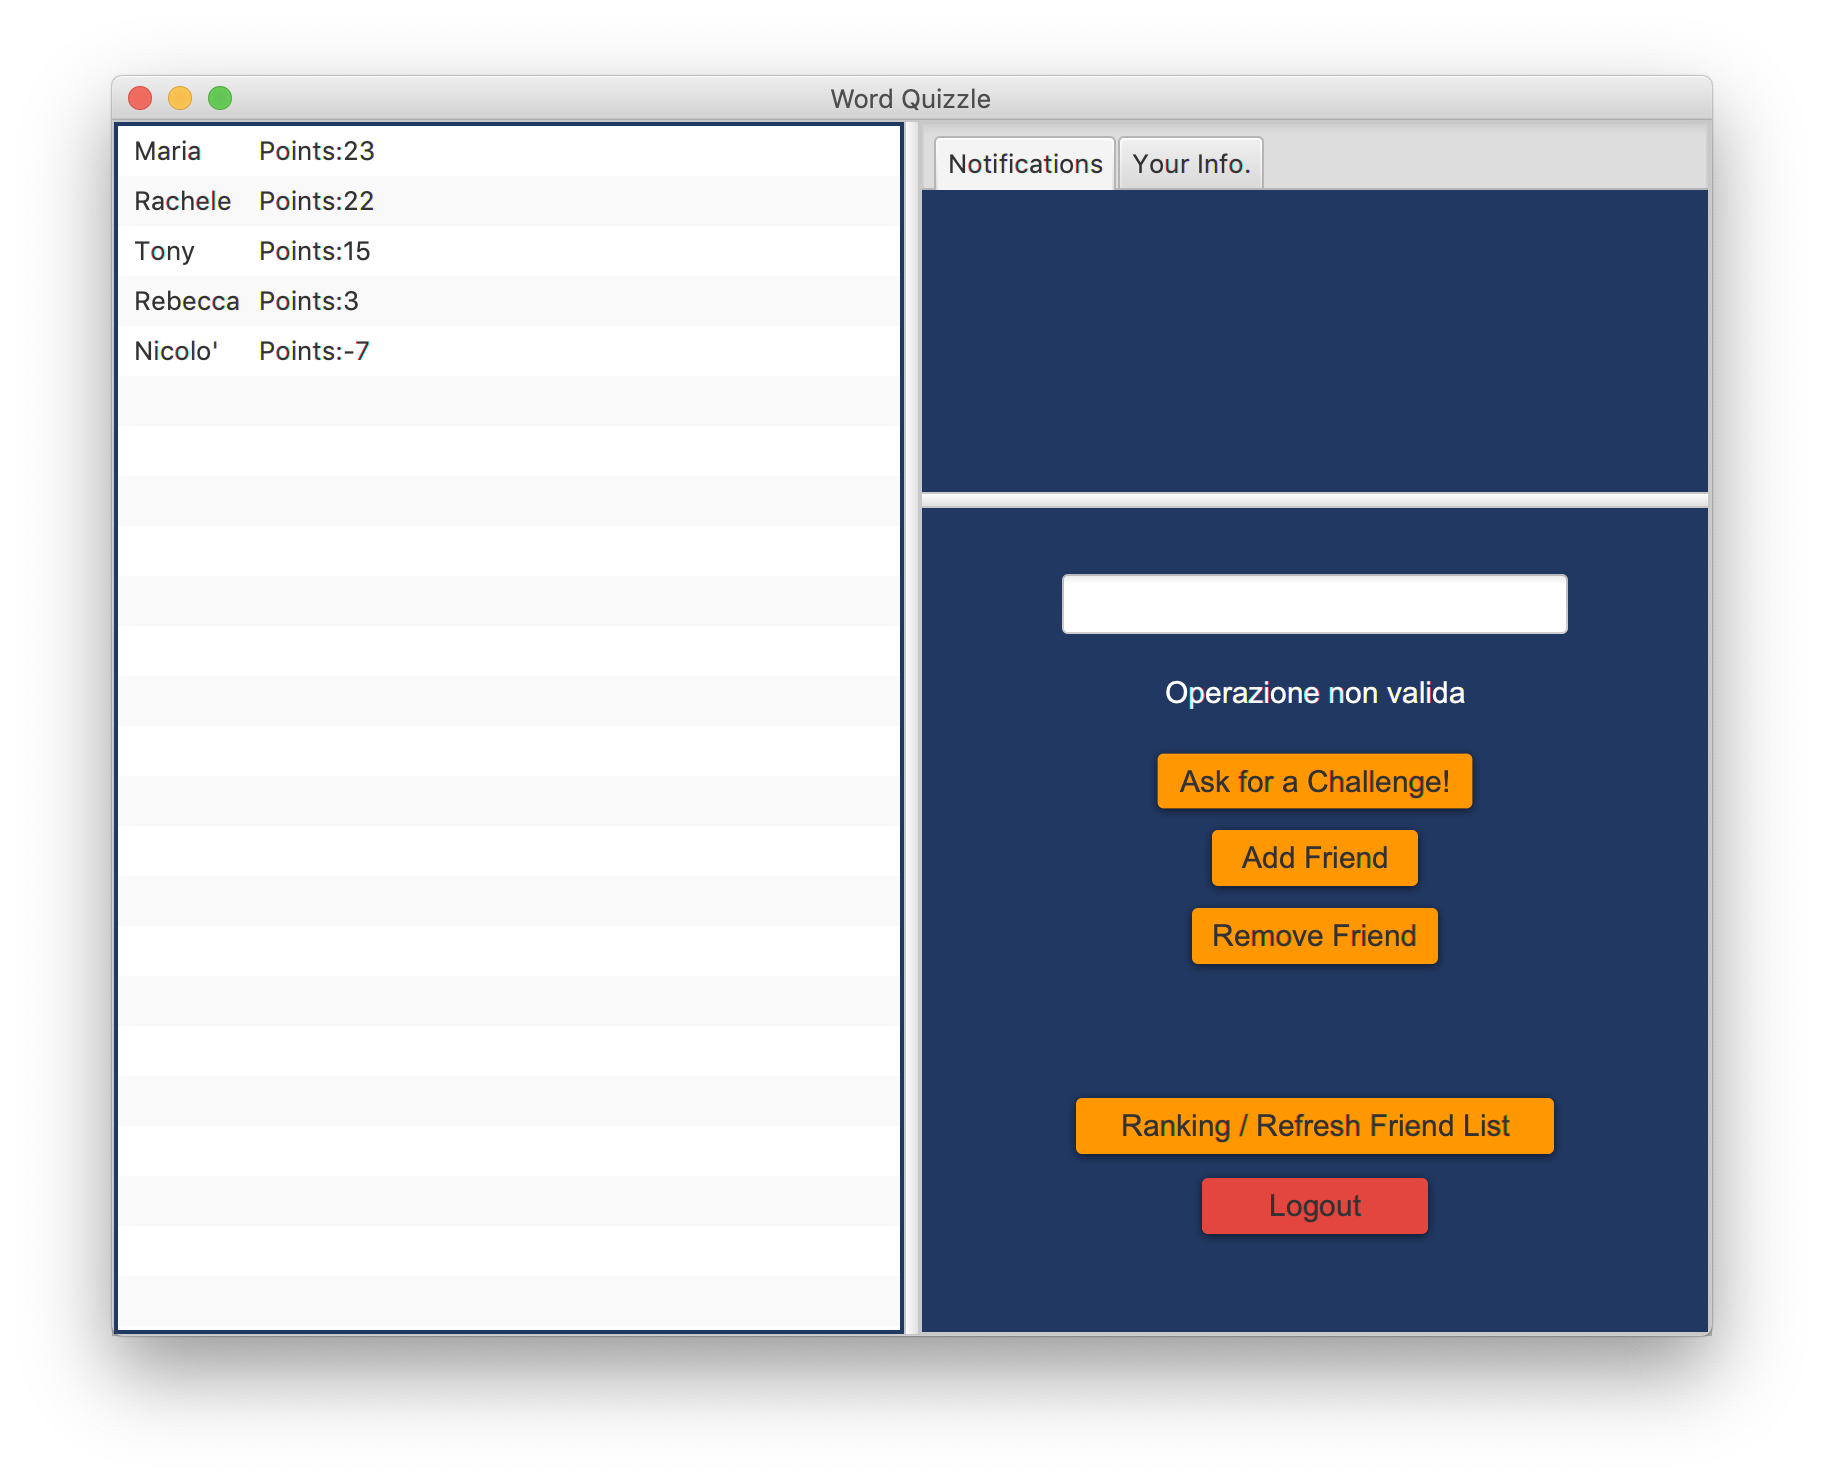
\includegraphics[scale=0.5]{quizzlemain.png}
\end{center}
Il controller della schermata principale è divisa in due parti, nella parte sinistra è presente una ListView di amici che possono essere aggiunti o rimossi grazie alla TextField e ai bottoni presenti nella parte destra. La ListView può essere settata in modalità classifica o lista di amicizie usando il Toggle apposito nella parte destra.
Nella parte destra superiore sono presenti due Tab, una per le notifiche e una contenente le informazioni correnti del utente (username e punteggio).
Ogni tasto si occupa di chiamare il metodo "handler" associato definito in WQClient (come già visto). Il metodo invierà al server tutti i comandi seguendo il protocollo e nel caso di errore si aggiorna la Label di errore posizionata sotto la TextField.
\clearpage

\section{Sfida}
Prima di illustrare la sfida è bene definire il thread che gestisce le notifiche lato client.

\subsection{WQNotify}
E' una classe client-side che si occupa di gestire tutte le notifiche che arrivano tramite UDP. Il Thread viene fatto partire appena il client è riuscito a loggarsi con successo, ad esso viene passato come parametro la DatagramSocket creata dal thread che gestisce l'interfaccia grafica. La creazione della socket nel thread principale mi permette di poter eseguire la socket.close() quando il client esegue il logout, quindi nel thread delle notifiche catturare l'eccezione e terminare il processo. Il thread è bloccante sulla receive della socket, quando riceve un datagramma lo tokenizza e viene aggiornata la GUI in base al contenuto. Il suo principale compito oltre a quello di ricevere i datagrammi è rendere visibile o invisibile la tab delle notifiche associando alla notifica l'username dello sfidante ricevuto all'interno del datagramma.

\subsection{Protocollo Notifica}
\begin{wrapfigure}{l}{6cm}
\centering
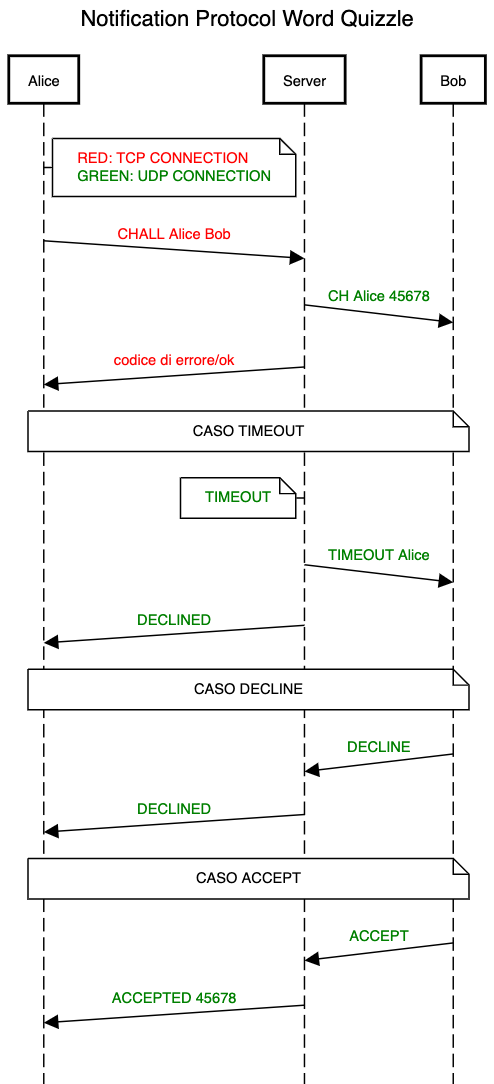
\includegraphics[width=6cm]{chprotocolscheme.png}
\end{wrapfigure}
Il protocollo di notifica ha inizio quando Alice manda a Bob, sotto connessione TCP standard, il messaggio "CHALL Alice Bob" che segue il protocollo di comunicazione standard definito dal server. Il server riceve il messaggio, lancia il thread della sfida creando una nuova socket TCP su una porta creata randomicamente (la chiameremo TCPport). Il server quindi invia sotto connessione UDP allo sfidato (Bob) il messaggio "CH Alice TCPport". Se l'invio della notifica è avvenuto con successo o ha riscontrato errori il server avvisa Alice tramite socket TCP standard. Il client di Bob, ricevuto il messaggio di sfida, aggiorna l'interfaccia grafica per mostrare la notifica.
Ci possiamo trovare quindi in 3 situazioni:
\begin{enumerate}
  \item Bob non risponde alla richiesta di sfida: la socket UDP del server non riceve risposta e scatta il timeout dopo il tempo T1. Il server invia "TIMEOUT" in un datagramma a Bob, che si occuperà di rimuovere la notifica aggiornando l'interfaccia grafica. Il server invia ad Alice "DECLINED" tramite UDP, che si occuperà di aggiornare la Label di errore e riattivare il tasto di richiesta di sfida.
  \item Bob non accetta la sfida: Bob invia il messaggio "DECLINE" al server e aggiornata la sua interfaccia grafica rimuovendo la notifica. Il server ricevuto il datagramma di Bob avvisa Alice inviando "DECLINED".
  \item Bob accetta la sfida: Bob invia al server "ACCEPT", il server poi spedisce ad Alice "ACCEPTED TCPport". Alice non era ancora a conoscenza della TCPport associata alla sfida.
\end{enumerate}
\clearpage
Una volta accettata la sfida per entrambi i giocatori si esegue uan chiamata al metodo gotoGame() di WQClient, ritrovandosi davanti la scena principale del gioco (GameView.fxml).

\subsection{Protocollo Sfida}
Messaggi inviati dal Server al Client:

\begin{table}[h]
\centering
\begin{tabular}{lllll}
parola\textunderscore ita  & var\textunderscore double \\
CHEND & punti\textunderscore ottenuti & parole\textunderscore corrette & parole\textunderscore errate & esito\textunderscore sfida \\
TIMEOUT & punti\textunderscore ottenuti & parole\textunderscore corrette & parole\textunderscore errate & esito\textunderscore sfida \\
\end{tabular}
\end{table}
\hfill \break
Messaggi inviati dal Client al Server:
\begin{table}[h]
\centering
\begin{tabular}{ll}
username & word\textunderscore eng \\
CHEXITED & \\
\end{tabular}
\end{table}

\subsection{WQChallenge on Server}
La classe WQChallenge rappresenta il thread dedicato alla sfida, viene lanciato dal thread che gestisce lo sfidante. Fa utilizzo del selector, è quindi un singolo thread che gestisce sequenzialmente entrambi i client (sfidato e sfidante). Il thread appena lanciato si occupa di scegliere randomicamente le K parole italiane dal file JSON "words.json" (le parole sono contenute in un JSONArray). A questo punto setta la socket TCP in modalità non bloccante e si mette in ascolto sulla select(). \\
Appena uno dei due client si collega, questo implica che la sfida è stata accettata, il thread si occupa di chiamare il servizio di traduzione per ogni parola italiana tramite API sfruttando la classe HttpsURLconnection e settando il metodo a "GET". La risposta che arriva dal servizio è una stringa JSON che va letta e analizzata con JSONParser fino a trovare la chiave "translatedText" che contiene come valore la traduzione più appropriata della parola italiana inviata. \\
Subito dopo aver tradotto le K parole viene fatto partire il timer della sfida (WQChallTimer), esso sfrutta la classe Timer e TimerTask definite in Java. Il loro compito è quello di eseguire il task (RemindTask) non appena il tempo richiesto è trascorso. Il il task si occupa semplicemente di incrementare una variabile volatile atomica per notificare al thread del selector che il tempo per la sfida è terminato.
\\
La chiave dopo l'accettazione è impostata in OP\textunderscore WRITE e viene allegata alla chiave una istanza di WQWord (definita nella prossima sottosezione). 

Se la chiave selezionata è in modalità scrittura viene inviata la parola italiana seguita da un valore "double", quest'ultimo è necessario al client per poter aggiornare la barra di avanzamento dell'interfaccia grafica.
Nel caso in cui uno dei due client termini (quindi la variabile volatile atomica "enduser" = 1) oppure le parole siano terminate (quindi l'indice contenuto nell'istanza di WQWord è maggiore K) o ancora nel caso in cui il timer sia scaduto (variabile atomica intera "to" = 1) il server invia il resoconto finale della sfida secondo Protocollo di sfida.

Se la chiave selezionata è in modalità lettura, il server legge la stringa inviata dal client e la analizza. se il testo corrisponde a "CHEXITED", significa che il client è uscito volotariamente dalla sfida quindi incrementa la variabile endusers e cancella la chiave dal selector. Se così non fosse, chiama il metodo "checkWords" che si occupa di controllare la correttezza della traduzione, aggiornando inoltre il puteggio dell'utente nel database principale e nella struttura delle statistiche associata alla chiave. Il server tiene conto della situazione in cui uno dei due client abbia terminato per primo (endusers = 1) non contando le parole inviate dall'ultimo client rimanente, inviando poi al ciclo successivo il messaggio di esito.

Al termine della sfida, dopo aver inviato entrmbi i messaggi di esito, il thread si occupa di aggiornare i punteggi anche sui file di persistenza.

\subsubsection{WQWord}
Di fondamentale importanza è la classe WQWord definita per poter aggiungere all' "attachment" della key (chiave del selector) le informazioni necessarie associate al client che sta giocando. La classe contiene variabile per identificare la parola da inviare, l'indice della parola e una classe ausiliaria "Statistics" necessaria per il calcolo delle statistiche finali della singola partita.

\subsection{GameViewController on Client}
\begin{center}
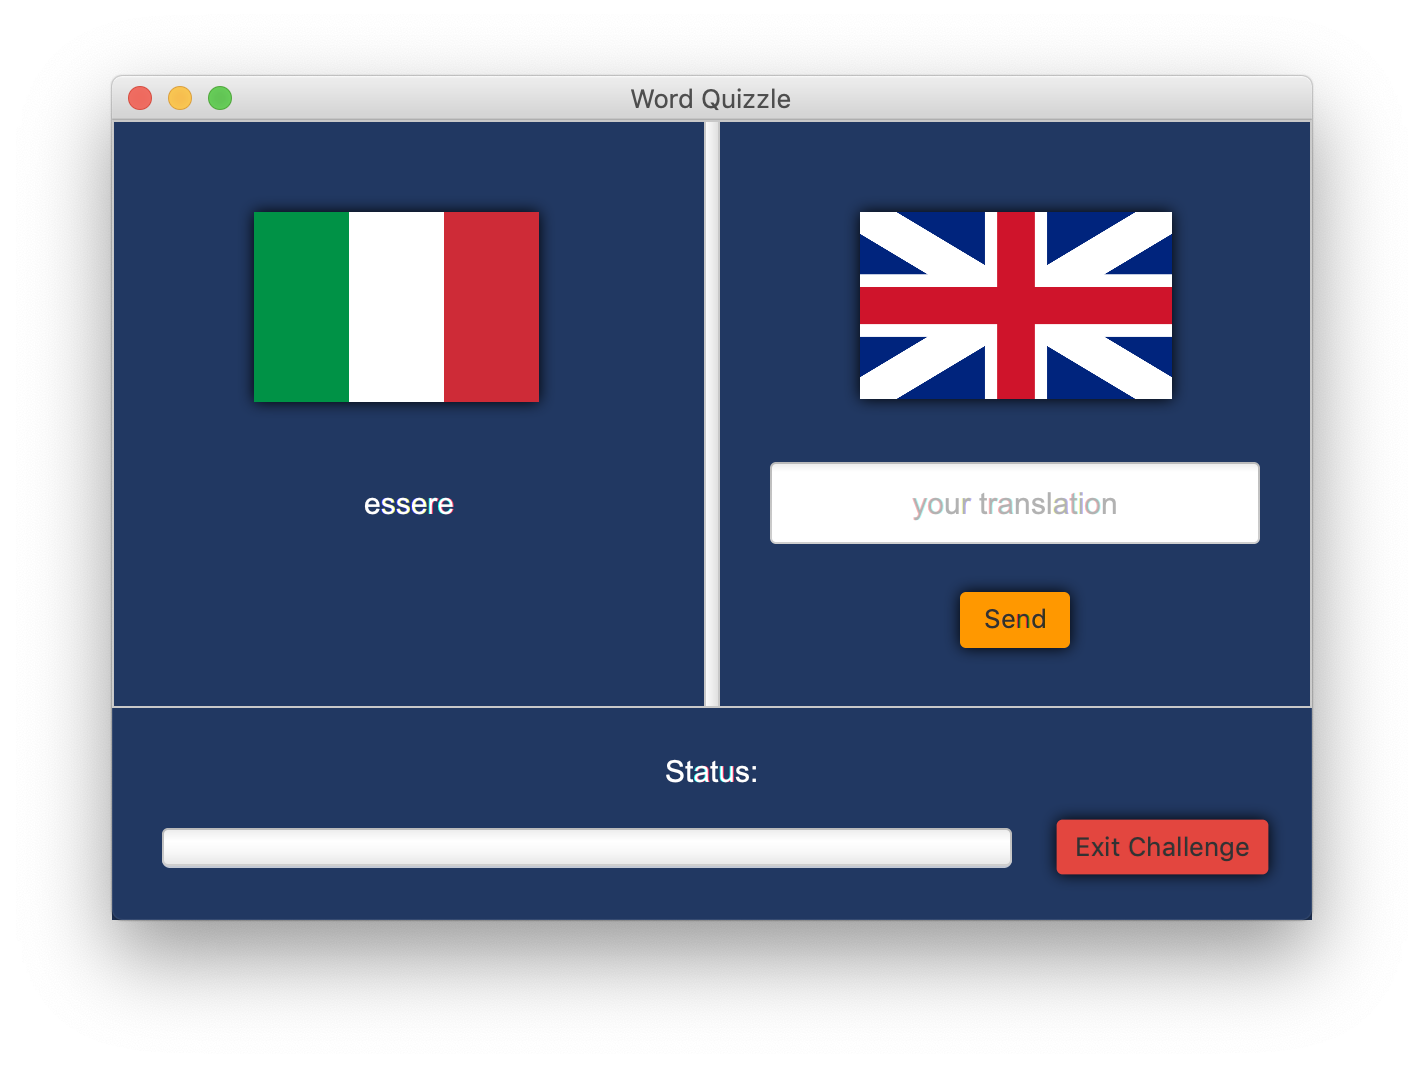
\includegraphics[scale=0.5]{quizzlegame.png}
\end{center}
Il Controller che si occupa del gioco è rappresentabile come una FSM con due stati: lettura e scrittura. Si trova inizialmente nello stato di lettura subito dopo aver effettuato la connessione TCP al server sulla porta della sfida. Avanza nello stato scrittura non appena viene cliccato il tasto di invio della parola e dopo l'invio del messaggio sulla socket TCP sfida, torna nello stato di lettura. Se il payload letto coincide con "CHEND" oppure "TIMEOUT" la sfida è terminata, quindi aggiorna l'interfaccia grafica con l'esito finale. Il client a questo punto attende che l'utente clicchi sul tasto di uscita dalla sfida, per inviare al thread della sfida "CHEXITED" ed infine settare la scena della schermata principale.

% Adding a bibliography if citations are used in the report
\bibliographystyle{plain}
\bibliography{bibliography}

\end{document}
